\documentclass[a4paper, 12pt]{article}
\usepackage[utf8]{inputenc}
\usepackage[english]{babel}
\usepackage[T1]{fontenc}
\usepackage{setspace}
\usepackage{hyperref}
\usepackage[top=3cm, bottom=3cm, left=3cm, right=3cm]{geometry}
\usepackage{color}
\usepackage{color, colortbl}
\usepackage{graphicx}
\usepackage{subcaption}
\usepackage{caption}
\usepackage{fancyhdr}
\usepackage{wrapfig}
\usepackage{appendix}
\usepackage{enumitem}
\usepackage{pifont}
\usepackage{hyperref}
\usepackage{amssymb,mathtools}
\usepackage{listings}
\definecolor{Gray}{gray}{0.9}
\usepackage{xcolor}

\definecolor{codegreen}{rgb}{0,0.6,0}
\definecolor{codegray}{rgb}{0.5,0.5,0.5}
\definecolor{codepurple}{rgb}{0.58,0,0.82}
\definecolor{backcolour}{rgb}{0.95,0.95,0.92}

\lstdefinestyle{mystyle}{
    backgroundcolor=\color{backcolour},   
    commentstyle=\color{codegreen},
    keywordstyle=\color{magenta},
    numberstyle=\tiny\color{codegray},
    stringstyle=\color{codepurple},
    basicstyle=\ttfamily\footnotesize,
    breakatwhitespace=false,         
    breaklines=true,                 
    captionpos=b,                    
    keepspaces=true,                 
    %numbers=left,                    
    %numbersep=5pt,                  
    showspaces=false,                
    showstringspaces=false,
    showtabs=false,                  
    %tabsize=2
}

\lstset{style=mystyle}

%bibliographie
\usepackage[
   backend=biber,        % compilateur par défaut pour biblatex
   sorting=nyt,          % trier par nom, année, titre
   citestyle=authoryear, % style de citation auteur-année
   bibstyle=alphabetic,  % style de bibliographie alphabétique
]{biblatex}
\addbibresource{mon-fichier-biblio.bib}




% Bandeau
\setcounter{tocdepth}{10}
\pagestyle{fancy}
\renewcommand\headrulewidth{1pt}
\fancyhead[R]{D.Grazzani, R.Grossoni}
\fancyhead[L]{
\includegraphics[width=2.5cm]{logo-mini polimi.jpg}}




\begin{document}
\noindent

%Page de titre

\begin{titlepage}

\begin{center}
\hspace{100cm}

\vspace{1cm}

\LARGE{\textbf{EMBEDDED SYSTEMS}}

\vspace{1cm}

\huge{\textbf{ Triple Redundancy Module On FreeRTOS}}

\vspace{1cm}

\LARGE{Davide Grazzani, Riccardo Grossoni }

\vspace{1cm}

\LARGE{Professors : William Fornaciari, Federico Reghenzani, Davide Baroffio}

\vspace{0,5cm}


\begin{figure}[h]
\begin{center}

\includegraphics[scale=1]{Logo_Politecnico_Milano.svg_.png}
\end{center}
\end{figure}

\vspace{1cm}



\end{center}

\end{titlepage}



\newpage
\tableofcontents
\newpage
\begin{onehalfspace}

\section{Introduction}
FreeRTOS is a lightweight real-time operating system designed for embedded systems. It manages tasks, which are independent units of execution, allowing multitasking by switching between them based on priority.
The objective of this project is to introduce a task-level, software-based method of recovering the correct execution after a single-time failure that extends the original FreeRTOS kernel.

Such recovery method in FreeRTOS is essential for ensuring system reliability and resilience, especially in environments where single-time failures can lead to critical malfunctions or data loss. By implementing recovery mechanisms within tasks, the system can detect and address failures locally, reducing the need for full system resets and maintaining overall system stability.

This project has been developed for the course \textit{Embedded Systems} at Politecnico di Milano.
% maybe change the word method to another “cleaner” word


\section{Structure and Functionality of the module}\label{section:how_does_it_works}
 In this section, changes to tasks and other elements of the kernel will be explained, to highlight how the recovery process works and how it impacts task management and execution; but first, let’s introduce how the process functions.
\subsection {High-level functionality description}
When a task is created using the new task creation function \texttt{xTaskCreateRedundant} (\ref{task_creator}), an identical "twin" task is also created, which from now on will be called Validation Task. Under normal behavior, both tasks are executed and should perform the same instructions, generating the same output.

These two outputs are checked after one iteration (when \texttt{vTaskDelay} or \texttt{xTaskDelayUntil} is called) and if they match, the execution continues normally. 

If a mismatch is detected, the recovery process will be started, which re-executes the iteration, checks if no error was found in this “re-execution” and restores the two tasks (the original and the validation task) to a correct state. 
\subsection {Task Control Block Changes}
Before showing the changes in the code, mind that usage of this module can and should be done by only referring to the API explained in chapter \ref{section:User Interface}. The following code has the only objective of helping the reader understand the internal structure of the module.
\begin{lstlisting}[language=C]
    #if (configUSE_REDUNDANT_TASK == 1)
        BaseType_t isRedundantTask;                    
        xRedundantStruct_t redundantStruct;            
    #endif\end{lstlisting}
These two entries are the modifications made on the Task Control Block. The first variable is a flag that states if a task is redundant (meaning that it has an associated Validation Task) or not, by assuming the value \texttt{pdTRUE} or \texttt{pdFALSE} respectively. The second variable is a structure containing all the relevant information associated with the redundancy feature.
\\
The definition of the type \texttt{xRedundantStruct\_t} is made inside the new file \texttt{redundancy.h}:
\begin{lstlisting}[language=C]
typedef struct xRedundantStruct {
        xRedundantShared_t * pxRedundantShared;        
        struct tskTaskControlBlock * pxTaskValidation; 
        struct tskTaskControlBlock * pxTaskSUS;        
        uint64_t iterationCounter;                     
        void * pxInputStruct;                          
        void * pxOutputStruct;                         
    } xRedundantStruct_t;
    \end{lstlisting}         
Leaving \texttt{pxRedundantShared} for last, the two TCB pointers \texttt{pxTaskValidation} and \texttt{pxTaskSUS} point respectively at the Validation Task and Recovery Task. Note that under normal behavior \texttt{pxTaskSUS} points to \texttt{NULL}, as there is no active recovery process. \\
The \texttt{iterationCounter} is an internal counter that marks at which iteration each task is, in order to synchronize each task with their validation.\\
The \texttt{pxInputStruct} and \texttt{pxOutputStruct} variables are pointers to the respective Input and Output structures of the task. Refer to chapter \ref{section:IO structure and Commit} for an explanation on their use.
 \begin{lstlisting}[language=C]
 typedef struct xRedundantShared {
        void (*pxCommitFunction)(void*);               
        void *pxCommitFunctionParameter;               
        void * pxSharedInputStruct;                  
        UBaseType_t uInputStructSize;                  
        UBaseType_t uOutputStructSize;                 
        BaseType_t isRecoveryProcess;                  
        TaskFunction_t taskCode;                       
        uint32_t stackDepth;                           
        void * pvParameters;                           
        void * pxCommitInputStruct;                    
        void * pxSharedOutputStruct;                  
    } xRedundantShared_t;
\end{lstlisting}
As the name suggests, xRedundantShared is a structure that is shared by the two "twin" tasks. It contains information used when creating the recovery task and when performing the error detection.\\ Additionally, it contains the reference to the commit function and its possible parameters, which is called when the error detection finds no errors and the generated output of the task must be committed. More information about the commit function can be found in chapter \ref{section:IO structure and Commit}. \\
\textbf{N.B.} Given a task and its "twin" task, their \texttt{pxTaskValidation} point to the other task, as each task sees its "twin" as the validation task.\\
\subsection{Commit Function, Input and Output Structures} \label{section:IO structure and Commit}
The commit function and the Input and Output structures are the 3 main elements that must be partially handled by the end-user through the API. In this section the Why, When and How they are used will be explained.
\begin{itemize}
    \item \label{trm:input_structure}{Input Structure: The input structure is a \texttt{struct} created by the end-user that contains all the data that should be available at the start of a task iteration. Through the use of the API the structure is linked to the correct task and a copy is created for the Validation task. At the end of each iteration, the input for the next iteration should be prepared, in order to be validated. After validation, a copy of the input is (automatically) saved in the shared structure, to be used in case of recovery. Refer to the first example for a clear and simple way on how to implement the input structure correctly (\ref{example:fibo}).
    }
    \item \label{trm:output_structure}{Output Structure: Similarly to the input structure, the Output structure is also created by the end-user. Differently from the input, the output will be filled by data obtained during the task execution, so during task initialization is important to just use the API function to \textit{allocate} the space needed for the structure. In the task body the output for the current iteration is then stored in the structure, which is validated at the end of the iteration. If no error is detected this output is then committed using the commit function. As for the input structure, a clear and simple example is available here (\ref{example:fibo}).
    }
    \item \label{trm:commit_function}{Commit Function: The commit function is the way a task actually outputs its data externally (as console prints, electrical signals, inputs for other tasks etc.). It's defined by the end-user and is only executed one time per iteration, after the validation step is completed successfully. While it's possible to use different data structures  from the output structure, it's good practice to just stick with that (to ensure that the data is consistent).
    }
\end{itemize}
As briefly introduced in the Commit function section, the input structure can be updated externally (meaning not from inside the task body). This comes with limitations; Since the end-user does not have access to the "twin" task, normally altering directly the input structure leads to mismatches during validation. To avoid this problem there's an available API function called \texttt{xSetTaskInput} (\ref{external_input}). This updates both tasks inputs, but it's performed only after the next successful commit step.
\subsection{Recovery Process}\label{trm:recovery_process}
In this section a detailed explanation of how the recovery process actually work will be made. Each of the following steps is completely hidden from the end-user, but it can be useful to learn how it works to better use this module. To further help with the understanding, there will be three subsections, the validation phase (\ref{validation_phase}), the recovery initialization phase (\ref{recovery_init_phase}) and the recovery ending phase (\ref{recovery_end_phase}).
\subsubsection{Validation Phase}\label{validation_phase}
\begin{figure}[h]
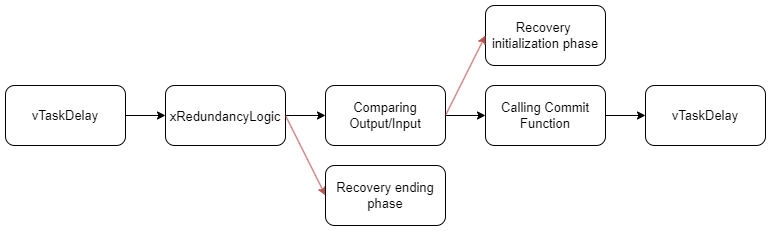
\includegraphics[width=\textwidth]{images/validation phase.png}
\caption{Validation phase}
\end{figure}
Once \texttt{vTaskDelay} is called (or \texttt{xTaskDelayUntil}), if the iteration counters of the current task and its validation task are equal the function \texttt{xRedundancyLogic} is called. Firstly it checks if the task was currently in recovery mode, and if it was the proper functions (see \ref{recovery_end_phase}) are called. If not, it means that an iteration has just finished, so it must be validated. Through the function \texttt{compareZone}, the current output and the input for the next iteration are validated between the two tasks. If \texttt{compareZone} detects any mismatch, then an error has occurred and the functions for the recovery initialization phase are called (see \ref{recovery_init_phase}). If no error is detected the commit function is called and the output is committed. After that if there is an external input update the input is updated and the function \texttt{xRedundancyLogic} returns with a \texttt{pdPASS} value.
\subsubsection{Recovery Initialization Phase}\label{recovery_init_phase}
\begin{figure}[h]
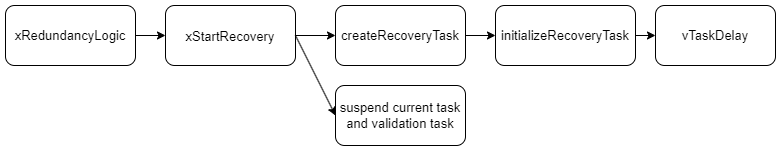
\includegraphics[width=\textwidth]{images/recovery init phase.png}
\caption{Recovery Initialization phase}
\end{figure}
When during the execution of the function \texttt{xRecoveryLogic} an error is detected in either the next input or the output, then the function \texttt{xStartRecovery} is called. This function suspends the current task and it's associated validation task, then it calls the function \texttt{createRecoveryTask}. This function handles the correct creation of the recovery task, then calls the \texttt{initializeRecoveryTask} for the initialization. \texttt{initializeRecoveryTask} sets all the correct settings for the recovery task, including the saved input structure at the last correct iteration. After the recovery task is created and initialized the scheduler resumes normally, and the recovery mode for the current task is maintained until the recovery task completes one iteration.
\subsubsection{Recovery Ending Phase}\label{recovery_end_phase}
\begin{figure}[h]
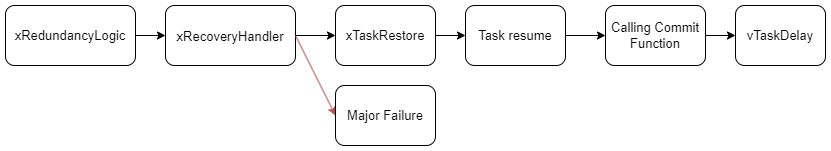
\includegraphics[width=\textwidth]{images/recovery end phase.png}
\caption{Recovery Ending phase}
\end{figure}
After the recovery task has performed one iteration, it will be on the same iteration count as the tasks where the error has been detected. At this point the \texttt{xRecoveryLogic} function calls the \texttt{xRecoveryHandler} function. This function compares the recovery task with the two "original" tasks, to find where the error is located, then it calls the \texttt{xTaskRestore} function, which updates the values of the erroneous task. The two original tasks are then resumed and the now correct output is committed. The recovery process is finished so the flag is updated and the program continues normally.\\
It's possible that the recovery process was not successful, meaning that during the \texttt{xRecoveryHandler} no correct task is found. In this case, the default behaviour of the program is to stall, but depending on the specific program it's possible to change this event by modifying accordingly the reserved macro hook. An explanation on how to perform that is left for the Advanced function section (\ref{defaultDelayFailureHandler}).
\subsection {Performances}\label{performances}
When considering performances, obviously the performances are at least halved, since this module adds an additional task that performs the same operations a second time. Having considered that, the actual additional overhead that this module adds is caused by the controls during the validation phase and the controls during the \texttt{traceTASK\_SWITCHED\_IN} macro (used for controlling task starvation). This means that the overhead strictly depends on the size of the input and output structures. Given that, testings with very large structures (array of 1000 integers) resulted in an overhead of single digit milliseconds ($\approx 8ms$ total, with 1000 iterations). Practically, tasks with higher delay will not be affected in a significant manner.\\
\textbf{N.B.}: The results reported above are entirely caused by the additional overhead of the validation and starvation controls.\\ \\
Highly repetitive tasks are what works best with this module, since the code will be fairly simple to translate without changing the entire structure and the temporal complexity can be easily determined.
\subsection{Limitations}\label{limitations}
As for the current version of the module, Notifications and queues are not supported with redundant tasks. Note that they can still be used with default tasks.\\
This is a single failure recovery module. This means that if a second failure happens \underline{\textbf{before}} the recovery mode successfully fixes the first error, then the behavior is not guaranteed. \\
Due to the use of task states such as \texttt{suspend} and \texttt{resume}, using such states can, in rare cases, lead to unexpected behavior. In particular, calling a \texttt{vTaskResume} on a task currently in recovery mode, will lead to the task remaining suspended. This is done to avoid resuming a task currently containing an error.\\
The hook \texttt{traceTASK\_SWITCHED\_IN} is used to manage task synchronization and starvation. Please refer to the advanced function section (\ref{traceTASK_SWITCHED_IN}) to learn how to extend it for other purposes.\\
Please consider that the redundancy feature uses around double the memory of a default task, due to the presence of the validation task. 
\section{User Interface} \label{section:User Interface}
In this section the interface available to end-user will be presented. Methods will be presented by usage domain.\\
\textbf{N.B.}: to use any redundant feature present in this kernel you must set \texttt{configUSE\_REDUNDANT\_TASK} to \texttt{1} in your \texttt{FreeRTOSConfig.h} config file.
\subsection{Task Creation \& Initialization}
In this sub-section function related to task creation and initialization are reported. It's important to note that these \underline{functions} should be \underline{called once and only once per task} and should anyway be \underline{called before \texttt{vTaskStartScheduler} function}\footnote{If you are using \texttt{CMSIS} library then the function is called \texttt{osKernelStart}}. Any eventual deviation from these guidelines will be specified in the function description itself.
\begin{itemize}
    \item \label{task_creator}{
        \begin{lstlisting}[language=C]
BaseType_t xTaskCreateRedundant( TaskFunction_t pxTaskCode,
    const char * const pcName,
    const configSTACK_DEPTH_TYPE usStackDepth,
    void * const pvParameters,
    UBaseType_t uxPriority,
    TaskHandle_t * const pxCreatedTask ) PRIVILEGED_FUNCTION;
        \end{lstlisting}
        This function creates a new redundant task. As you may notice, the signature of this function is exactly the same as \texttt{xTaskCreate}\footnote{Please refer to the FreeRTOS documentation if you need more insight  \ref{url:freertos_doc}}, hence the data needed to initialize a redundant task is no different from a default task.
    }
    \item {
        \begin{lstlisting}[language=C]
BaseType_t xSetInput(TaskHandle_t task, void* pxStruct, UBaseType_t uxSize);
        \end{lstlisting}
        This function sets the input structure(\ref{trm:input_structure}) \texttt{pxStruct} into a task given its own TaskHandle \texttt{task} and the size of the input structure \texttt{uxSize}. The input structure represent a custom user-defined data structure containing all the information needed for such a task to execute correctly a job. The input structure should be defined by the user based on the need of the task and should be correctly initialized before passing it to this function.
    }
    \item{
        \begin{lstlisting}[language=C]
BaseType_t xSetOutput(TaskHandle_t task, UBaseType_t uxSize);
        \end{lstlisting}
        Similar to \texttt{xSetInput}, this function sets the output structure(\ref{trm:output_structure}) size \texttt{uxSize} into a task given its own TaskHandle \texttt{task}. \\
        \textbf{N.B.}: here the structure initialization is not needed\footnote{It's declaration is advised in order to obtain the size using \texttt{sizeof()} function.} as the kernel already handles the initialization. Moreover, this call is optional.
    }
    \item {
        \begin{lstlisting}[language=C]
BaseType_t xSetCommitFunction(TaskHandle_t task, void (*pxCommitFunction)(void*), void* pxCommitFunctionArgs);
        \end{lstlisting}
        This function sets a custom function \texttt{pxCommitFunction} ( and eventually the function parameters \texttt{pxCommitFunctionArgs} ) to a given task \texttt{task} given the TaskHandle. The commit function is a method executed only after a successful check of the integrity of the task and should be used only for state-changing actions and operations.\footnote{An example of a state-changing action is a write on \texttt{UART}, the toggle of a led but also the changing of the state (i.e. suspend) of another task}
    }
\end{itemize}
\subsection{Task Control}
In this section all other APIs available to a redundant task are presented. Keep in mind that this APIs are all optional and are designed to facilitate the end-user workflow while building its application.
\begin{itemize}
    \item {
    \begin{lstlisting}[language=C]
void* xGetInput();
        \end{lstlisting}
        This function returns the input structure of a redundant task (the context is the current running task when the call is made). This method is useful when working inside the main body of a task and the user wants to retrieve the input structure of such a task.
    }
    \item {
    \begin{lstlisting}[language=C]
void* xGetOutput();
        \end{lstlisting}
        Similar to \texttt{xGetInput}, it returns the output structure of a redundant task. 
    }
    \item \label{external_input}{
    \begin{lstlisting}[language=C]
void xSetTaskInput(TaskHandle_t task, void* pxStruct);
        \end{lstlisting}
        Method used to modify the flow of a redundant task. Given a TaskHandle \texttt{task} and a compatible input structure \texttt{pxStruct}, the kernel sets such a structure as the \underline{the next input of the task}. It's worth to be noted that the \underline{input is set only after a successful commit has happened, not immediately}. This function is useful to synchronize operations between tasks.
    }
    \item {
    \begin{lstlisting}[language=C]
void* xGetTaskOutput(TaskHandle_t task);
        \end{lstlisting}
        Given a \texttt{task}, this function returns the output structure of a redundant task \underline{updated to the last commit}. This method is useful to synchronize operations between tasks.
    }
\end{itemize}
\subsection{Advanced function}
In this section advanced function \underline{that should only be touched by experienced FreeRTOS} \underline{users} are presented. Keep in mind that every modification or override of this function may leave the system in a non-functional state or break redundancy mechanisms.
\begin{itemize}
    \item {
    \begin{lstlisting}[language=C]
BaseType_t defaultRecoveryHandler();
        \end{lstlisting}
        Default implementation of the recovery behavior  during a system event (namely every vTask\* call that happens during a recovery phase). It's possible to override this function by setting \texttt{traceTASK\_RECOVERY\_MODE()} in \texttt{FreeRTOS.h} file.
    }
    \item \label{traceTASK_SWITCHED_IN}{
    \begin{lstlisting}[language=C]
void xSuspendTaskAhead();
        \end{lstlisting}
        Default implementation of the \texttt{traceTASK\_SWITCHED\_IN()} that prevent racing condition in the context of the same redundant task (effectively preventing starving). It's possible to extend (or even override, discouraged) this function in \texttt{tasks.c} file.
    }
    \item \label{defaultDelayFailureHandler} 
    {
        \begin{lstlisting}[language=C]
void defaultDelayFailureHandler();
        \end{lstlisting}
    Default implementation of how the system behaves in case of a major failure (a second error occurring before the first one is fixed). The default implementation stalls the system, override is possible.
    }
\end{itemize}
\newpage

\section{Example}
In this section two examples will be presented: a trivial example on the Fibonacci sequence (\ref{url:fibonacci_sequence}) that aims to touch all the basic functionality of the redundant kernel, and another one using Ascon (\ref{url:ascon}, \ref{url:ascon_code}), a lightweight family of encryption, decryption and hashing algorithms. In this latter example a more \textit{"realistic"} use-case is presented, giving to the user a more meaningful example of usage of this kernel.\\
\textbf{N.B.}: all these examples where written and tested under Stm32's \texttt{Nucleo-L152re} board. Moreover \texttt{CMSIS v2} (\ref{url:cmsis_v2}) interface was used.
\subsection{Example 1: Fibonacci Sequence} \label{example:fibo}
If you are not familiar with the Fibonacci sequence take a look at this (\ref{url:fibonacci_sequence}) first.\\
\begin{enumerate}
    \item {
    Definition of the task:
        \begin{lstlisting}[language=C]
// global scope

// using default CMSIS v2 interface to define a new task
osThreadId_t taskFibonacci;
const osThreadAttr_t taskFibonacciAttributes = {
  .name = "fiboTask",
  .stack_size = 500 * 4,
  .priority = (osPriority_t) osPriorityNormal,
};

// define input and output structure
typedef struct inputFibonacci {
  int n_previous;
  int n_current;
} inputFibonacci_t;

typedef struct outputFibonacci {
  int n_next;
} outputFibonacci_t;

//define a commit function
void commitFibonacci(){
  outputFibonacci_t * output = (outputFibonacci_t*) xGetOutput();
  printf("output FIBONACCI [COMMIT] : %d\n", output->n_next);
}

// declare the main body of the task
void taskFibonacciBody(void *argument);
        \end{lstlisting}
        As you can see here we have defined 2 structure, one for the input and one for the output.
        In the input structure stores $F_{n-1}$ and $F_{n-2}$ meanwhile the output structure stores $F_n$. It's important to be noted, as discussed in section \ref{section:how_does_it_works}, that at each iteration the output should be entirely generated again. We will better this concept in a few steps. We also define the \texttt{commitFibonacci} function, a method executed only after each successful commit. In this case the function retrieves the output by calling \texttt{(outputFibonacci\_t*) xGetOutput()} (note the required cast!) and subsequently proceeds to print the output.
    }
    \item {
    Creation of the task:
    \begin{lstlisting}[language=C]
// in the main function

/* Init scheduler */
osKernelInitialize();
  
//initializing taskFibonacci
// here osThreadNewRedundant it's only a wrapper of xTaskCreateRedundant, code available on References and Material
taskFibonacci=osThreadNewRedundant(taskFibonacciBody, NULL, &taskFibonacciAttributes);

//initializing the input of the task
inputFibonacci_t * input_og = pvPortMalloc(sizeof(inputFibonacci_t));
input_og->n_previous = 0;
input_og->n_current = 1;
xSetInput(taskFibonacci, input_og, sizeof(inputFibonacci_t));

//setting the output
xSetOutput(taskFibonacci, sizeof(outputFibonacci_t));

//setting the commit function
xSetCommitFunction(taskFibonacci, commitFibonacci, NULL);

/* Start scheduler */
osKernelStart();
        \end{lstlisting}
        Here we create the task using \texttt{osThreadNewRedundant} (\ref{code:osthreadnewredundant}), a wrapper function for \texttt{xTaskCreateRedundant}.
        Once the task is created, we proceed to initialize the input as required by the Fibonacci sequence ($F_0 = 0$ and $F_1 = 1$) and then setting the output.
        We tell the kernel not the actual values of the output (in fact as you can see no initialization of the structure is required) but instead only the size the kernel should reserve for the output itself. Subsequently by calling \texttt{xSetCommitFunction} we link the commit function to the task itself.
        \texttt{osKernelStart} starts FreeRTOS.\\
        \textbf{N.B.}: it's imperative to call \texttt{xSetInput} once and before \texttt{osKernelStart}, \texttt{xSetOutput} it's optional but should be included in the same scope of \texttt{xSetInput}. \texttt{xSetCommitFunction} instead can be called multiple times either in the \texttt{main} scope or in the \texttt{task-body} scope.
    }
    \item {
    Task body:
    \begin{lstlisting}[language=C]
void taskFibonacciBody(void *argument){

  //-- header of the task --
  int result;
  outputFibonacci_t * output;
  inputFibonacci_t * input;

  //-- main for loop --
  for(;;){

    // just making sure every loop cycle the correct pointers are fetched
    // this is not strictly necessary, could be moved to the header of the task
    input = (inputFibonacci_t*) xGetInput();
    output= (outputFibonacci_t*) xGetOutput();

    // calculating new output
    result = input->n_previous + input->n_current;
    output->n_next = result;

    //updating previous input for the next cycle
    input->n_previous = input->n_current;
    input->n_current = output->n_next;

    // calling osDelay
    // at this point the task is suspended. Once the validation task reaches the same point in execution
    // of this task the health check is performed. Upon successful check, commit function taskFibonacci is executed.
    osDelay(5000);
  }
}      
    \end{lstlisting}
    Let's take a look to the main body of the Fibonacci task. In this example you can clearly distinguish two parts: the header of the task, the part of the function prior to the for-loop, and the main for-loop itself. It's important to clearly define this two areas of the task's body in order to assure a correct recovery process (\ref{trm:recovery_process}) in case of failure.
    \begin{itemize}
        \item {\textbf{Header of the task}: in this part of the function it's important \underline{to not to} \underline{write any static, non-conditional statements}. This is because the header of the task is a soft initialization zone, that gets executed every time a new task is spawned, hence also in case of error in the task. To understand better this concept we analyze our code:
        \begin{lstlisting}[language=C]
//-- header of the task --
int result;
outputFibonacci_t * output;
inputFibonacci_t * input;        
        \end{lstlisting}
        Here we only declare our variables but we do not initialize them until the body of the for-loop. If we were to initialize them we would need to make sure that, in case of error, the spawned task should initialize in a state which is at the same point of execution of the original task. From this consideration we should acknowledge:
        \begin{enumerate}
            \item The use of the input and output structure is fundamental as it has be designed to solve this specific problem
            \item Avoid local variables outside input and output structure if possible
            \item Pointers behave differently since they are stored in the heap so it's always possible to reference them, but you should then consider data integrity problem. Once again a possible solution is to use input and output structure.
        \end{enumerate}
        For the sake of completeness let's make a \textbf{WRONG example}:
            \begin{lstlisting}[language=C]
// WRONG EXAMPLE
void taskFibonacciBody(void *argument){

  //-- header of the task --
  int result;
  outputFibonacci_t * output;
  inputFibonacci_t * input;

  // this is fine.
  input = (inputFibonacci_t*) xGetInput();
  output= (outputFibonacci_t*) xGetOutput();

  // hard coded intialization BROKE RECOVERY
  input->n_previous = 0;
  input->n_current = 1;

  //-- main for loop --
  for(;;){
    //for loop code
  }
}      
    \end{lstlisting}
    In this example we first declare and get the input and output structure. You can safely call \texttt{xGetInput} and \texttt{xGetOutput} inside the header of the task as those are special function that do handle data integrity checks during recovery period (meaning that if an error occurs during the task execution this function will return prior-failure data).
    \begin{lstlisting}[language=C]
// hard coded intialization BROKE RECOVERY
input->n_previous = 0;
input->n_current = 1;
    \end{lstlisting}
    This however breaks the recovery process. This is due to the fact that at iteration $x$, when a failure happens, the value of the input structure should be restored to $x-1$ iteration, but they are overridden by those two upper lines of code resulting in a broken recovery process.
        }
    \item { \textbf{Main For-Loop of the task}: in this part of the function the implementation of the task's logic should be written. No particular recommendation should be made here, aside from the following:
    \begin{enumerate}
        \item {\texttt{osDelay} should be called every time a check with the validation task is needed, this is ideally once per loop cycle \underline{at the end of such a cycle}. This is because, in case of failure, the task should be able to go through at least a full iteration. }
        \item {The output structure should be entirely populated every iteration of the task, because in case of error during the execution, the \underline{entire} \underline{output structure} of the task is \underline{dirty}\footnote{In particular, old outputs might contain wrong data due to errors. This errors would not be restored by the recovery process, so they will remain even after a successful recovery, causing a cascade effect on future iterations.}. Let's take a look at this \textbf{WRONG example}:
        \begin{lstlisting}[language=C]
typedef struct inn {
    int a;
    int b;
    int counter;
} inn_t;

typedef struct outt {
    int a;
    int b;
} outt_t;

// in the task body
// assume a and b are initialized to 0
for(;;){
    if (i%2 == 0){
        inn->a++;
        out->a = inn->a;
    } else {
        inn->b++;
        out->b = inn->b;
    }
    inn->counter++;
    osDelay(1000);
}

    \end{lstlisting}
    In this example at iteration $x=2$ output structure holds \texttt{out->a = 1, out->b = 1}. In case of failure on the next step the output is wiped, and a re-execution would result in \texttt{out->a = 2, out->b = RANDOM\_ERROR} which is different from the correct result \texttt{out->a = 2, out->b = 1}, hence breaking recovery process. A solution to this problem would be this:
            \begin{lstlisting}[language=C]
// in the task body
// assume a and b are initialized to 0
for(;;){
    if (inn->counter%2 == 0){
        inn->a++;
    } else {
        inn->b++;
    }
    //always update the output at every iteration
    out->a = inn->a;
    out->b = inn->b;
    
    inn->counter++;
    osDelay(1000);
}

    \end{lstlisting}
    }
    \end{enumerate}
    
    }
    \end{itemize}
    }
\end{enumerate}

\subsection{Example 2: Ascon}
In this section a more practical example on how to develop using this kernel is presented. In this example we are going to develop a service able to encrypt and decrypt messages thanks to the Ascon library. If you are not familiar with Ascon implementation please see this (\ref{url:ascon_code}). Moreover we are also going to see how to perform communication with a redundant task.
\begin{itemize}
    \item {
    Task declaration
    \begin{lstlisting}[language=C]
// import ascon api headers
#include "api.h"
#include "ascon.h"
#include "crypto_aead.h"
#include "permutations.h"
#include "word.h"

// define our task that will query taskAscon
osThreadId_t taskUser;
const osThreadAttr_t taskUserAttributes = {
  .name = "UserTask",
  .stack_size = 1000 * 4,
  .priority = (osPriority_t) osPriorityNormal,
};

// ascon service
osThreadId_t taskAscon;
const osThreadAttr_t taskAsconAttributes = {
  .name = "AsconTask",
  .stack_size = 4000 * 4,
  .priority = (osPriority_t) osPriorityNormal,
};

// define the task bodies
void taskUserBody(void *argument);
void taskAsconBody(void *argument);

// define the commit functions
void commitAscon();

#define AD_LENGTH 16
#define M_LENGTH 64
#define EXEC_STATE_ACTIVE 1
#define EXEC_STATE_INACTIVE 0
#define EXEC_STATE_DONE 2
#define EXEC_MODE_ENCRYPT 1
#define EXEC_MODE_DECRYPT 0

//LIM: cannot use pointers inside this struct
typedef struct inputAscon {
  uint8_t exec_state;
  uint8_t exec_mode;
  unsigned char cypher[M_LENGTH + CRYPTO_ABYTES];
  unsigned long long cypher_len;
  unsigned char message[M_LENGTH];
  unsigned long long message_len;
  unsigned char ad[AD_LENGTH];
  unsigned long long ad_len;
  unsigned char nonce[CRYPTO_NPUBBYTES];
  unsigned char key[CRYPTO_KEYBYTES];
} inputAscon_t;

typedef struct outputAscon {
  uint8_t exec_state;
  uint8_t exec_mode;
  unsigned char cypher[M_LENGTH + CRYPTO_ABYTES];
  unsigned char message[M_LENGTH];
  unsigned long long cypher_len;
  unsigned long long message_len;
} outputAscon_t;

void commitAscon(){
  outputAscon_t * output = (outputAscon_t*) xGetOutput();
  if (output->exec_state == EXEC_STATE_DONE){
    if (output->exec_mode == EXEC_MODE_ENCRYPT){
      printf("OUTPUT Cypher: ");
      for (int i = 0; i < output->cypher_len; i++){
        printf("%02x", output->cypher[i]);
      }
      printf("\n");
    } else if (output->exec_mode == EXEC_MODE_DECRYPT){
      printf("OUTPUT Message: ");
      for (int i = 0; i < output->message_len; i++){
        printf("%02x", output->message[i]);
      }
      printf("\n");
    }
  }
}
    \end{lstlisting}
    In this part of the code our \textit{"user"} task and the Ascon task are defined. Input and output of the Ascon task are defined based on the input needed and the output produced by the original Ascon implementation of function \texttt{crypto\_aead\_encrypt} and \texttt{crypto\_aead\_decrypt}.
    }
    \item {
    Initialization
    \begin{lstlisting}[language=C]
taskAscon = osThreadNewRedundant(taskAsconBody, NULL, &taskAsconAttributes);  // in task.h xTaskCreateRedundant
taskUser = osThreadNew(taskUserBody, NULL, &taskUserAttributes); 

// setting the input of the ascon task
inputAscon_t * inputAscon = pvPortMalloc(sizeof(inputAscon_t));
inputAscon->exec_state = EXEC_STATE_INACTIVE;
xSetInput(taskAscon, inputAscon, sizeof(inputAscon_t));

// setting the output of the ascon task
xSetOutput(taskAscon, sizeof(outputAscon_t));

// set the commit function of the ascon task
xSetCommitFunction(taskAscon, commitAscon, NULL);
    \end{lstlisting}
    Here we create a default task \texttt{taskUser} and the redundant task \texttt{taskAscon}. Then the input of Ascon is initialized in a waiting state.
    }
    \newpage
    \item {
    User task body
    \begin{lstlisting}[language=C]
void taskUserBody(void *argument)
{
  // declarizing and initializing
  unsigned char message[M_LENGTH];
  unsigned char ad[AD_LENGTH];
  // some more code here
  //...

  // synch mechanism
  printf("\nAwaiting for the encryption service to be ready\n");

  // getting the task handle of taskAscon
  TaskHandle_t taskAscon = xTaskGetHandle("AsconTask");
  uint8_t ready = 0;
  
  // wait for the output of the ascon task to be set to inactive
  while (!ready){
    outputAscon_t * output = (outputAscon_t*) xGetTaskOutput(taskAscon);
    if (output->exec_state == EXEC_STATE_INACTIVE){
      ready = 1;
    }
    osDelay(50);
  }

  // preparing the input to the ascon task
  inputAscon_t * input = pvPortMalloc(sizeof(inputAscon_t));
  input->exec_state = EXEC_STATE_ACTIVE;
  // some more code here for initialization
  // ...

  // setting the input of the ascon task
  printf("Input set for encryption\n");
  xSetTaskInput(taskAscon, input);

  // function continues here by doing the same except calling for decrypt function
  // please see full version on examples/ascon_service

}
    \end{lstlisting}
    In this snippet of code we can appreciate sync mechanism using API call \texttt{xGetTaskOutput}, that conveniently contains the state of the Ascon service, to set at appropriate time a new input for the service using \texttt{xSetTaskInput}.
    }
    \item {
    Ascon task body
    \begin{lstlisting}[language=C]
void taskAsconBody(void *argument){
  inputAscon_t * input = (inputAscon_t*) xGetInput();
  outputAscon_t * output = (outputAscon_t*) xGetOutput();
  for(;;){
    // an external task has to set the input
    if(input->exec_state == EXEC_STATE_ACTIVE){

      if(input->exec_mode == EXEC_MODE_ENCRYPT){
        
        crypto_aead_encrypt(input->cypher, &input->cypher_len, input->message, input->message_len, input->ad, input->ad_len, NULL, input->nonce, input->key);
        input->exec_state = EXEC_STATE_DONE;
        output->exec_state = input->exec_state;
        output->exec_mode = input->exec_mode;

        output->cypher_len = input->cypher_len;
        memcpy(output->cypher, input->cypher, input->cypher_len);
        
      } else if(input->exec_mode == EXEC_MODE_DECRYPT){
        
        crypto_aead_decrypt(input->message, &input->message_len, NULL, input->cypher, input->cypher_len, input->ad, input->ad_len, input->nonce, input->key);
        input->exec_state = EXEC_STATE_DONE;
        output->exec_state = input->exec_state;
        output->exec_mode = input->exec_mode;
        output->message_len = input->message_len;
        memcpy(output->message, input->message, input->message_len);
      
      }

    } else if (input->exec_state == EXEC_STATE_DONE) {
      input->exec_state = EXEC_STATE_INACTIVE;
      output->exec_state = input->exec_state;
    }
    osDelay(50);
  }
}
    \end{lstlisting}
    In this function it's worth noting the structure of the main for-loop: it's written in a \texttt{if-else} conditional structure that does avoid ambiguity even in case of a failure during computation of either decryption or encryption. In this case, if a fault occurs, the task can simply repeat the process thanks to the encoding in the \texttt{inputAscon\_t} structure of the variable \texttt{exec\_mode}, effectively restoring original operational state.
    }
\end{itemize}

\section{References and additional material}
\begin{enumerate} 
    \item \textit{FreeRTOS Documentation}, \url{https://www.freertos.org/Documentation/00-Overview}\label{url:freertos_doc}
    \item \textit{Fibonacci Sequence}, \url{https://en.wikipedia.org/wiki/Fibonacci_sequence}\label{url:fibonacci_sequence}
    \item \textit{Ascon}, \url{https://ascon.iaik.tugraz.at}\label{url:ascon}
    \item \textit{Ascon C implementation}, \url{https://github.com/ascon/ascon-c}\label{url:ascon_code}
    \item \textit{CMSIS v2}, \url{https://arm-software.github.io/CMSIS_6/latest/RTOS2/index.html}\label{url:cmsis_v2}
    \item {\textit{osThreadNewRedundant implementation}
    \begin{lstlisting}[language=C]
osThreadId_t osThreadNewRedundant (osThreadFunc_t func, void *argument, const osThreadAttr_t *attr) {
  char empty;
  const char *name;
  uint32_t stack;
  TaskHandle_t hTask;
  UBaseType_t prio;

  hTask = NULL;

  if (!IS_IRQ() && (func != NULL)) {
    stack = configMINIMAL_STACK_SIZE;
    prio  = (UBaseType_t)osPriorityNormal;

    empty = '\0';
    name  = &empty;

    if (attr != NULL) {
      if (attr->name != NULL) {
        name = attr->name;
      }
      if (attr->priority != osPriorityNone) {
        prio = (UBaseType_t)attr->priority;
      }

      if ((prio < osPriorityIdle) || (prio > osPriorityISR) || ((attr->attr_bits & osThreadJoinable) == osThreadJoinable)) {
        return (NULL);
      }

      if (attr->stack_size > 0U) {
        /* In FreeRTOS stack is not in bytes, but in sizeof(StackType_t) which is 4 on ARM ports.       */
        /* Stack size should be therefore 4 byte aligned in order to avoid division caused side effects */
        stack = attr->stack_size / sizeof(StackType_t);
      }
      if (xTaskCreateRedundant ((TaskFunction_t)func, name, (uint16_t)stack, argument, prio, &hTask) != pdPASS) {
        hTask = NULL;
      }
    }
  }

  return ((osThreadId_t)hTask);
}
    \end{lstlisting}\label{code:osthreadnewredundant}}

\end{enumerate}

\end{onehalfspace}

\end{document}